\documentclass{article}
\usepackage[utf8]{inputenc}
\usepackage{amsmath}
\usepackage{amsthm}
\usepackage{amsfonts}
\usepackage{amssymb}
\usepackage{amstext}
\usepackage{gensymb}
\usepackage{graphicx}
%\usepackage{bbold}
%\usepackage{url}
%\usepackage{booktabs}
%\usepackage{marvosym}
%\usepackage{wasysym}
\pagenumbering{arabic}
\usepackage{fancyhdr}
\usepackage[margin=1.0in]{geometry}
\usepackage{eucal}

\usepackage{fancyvrb}

\def\N{\mathbb{N}}
\def\Z{\mathbb{Z}}
\def\Q{\mathbb{Q}}
\def\R{\mathbb{R}}
\newcommand{\Mod}[1]{\ (\text{mod}\ #1)}

\pagestyle{fancy}
\fancyhf{}
\rhead{MATH 4500}
\lhead{Alexander Winkles}
\chead{\Large \textbf{Computer Project 3}}
\cfoot{Page \thepage}

\begin{document}

\VerbatimInput{alexander_winkles_lab3.log}

\begin{figure}[H]
\centering
\caption{Polynomial interpolation when n = 5}
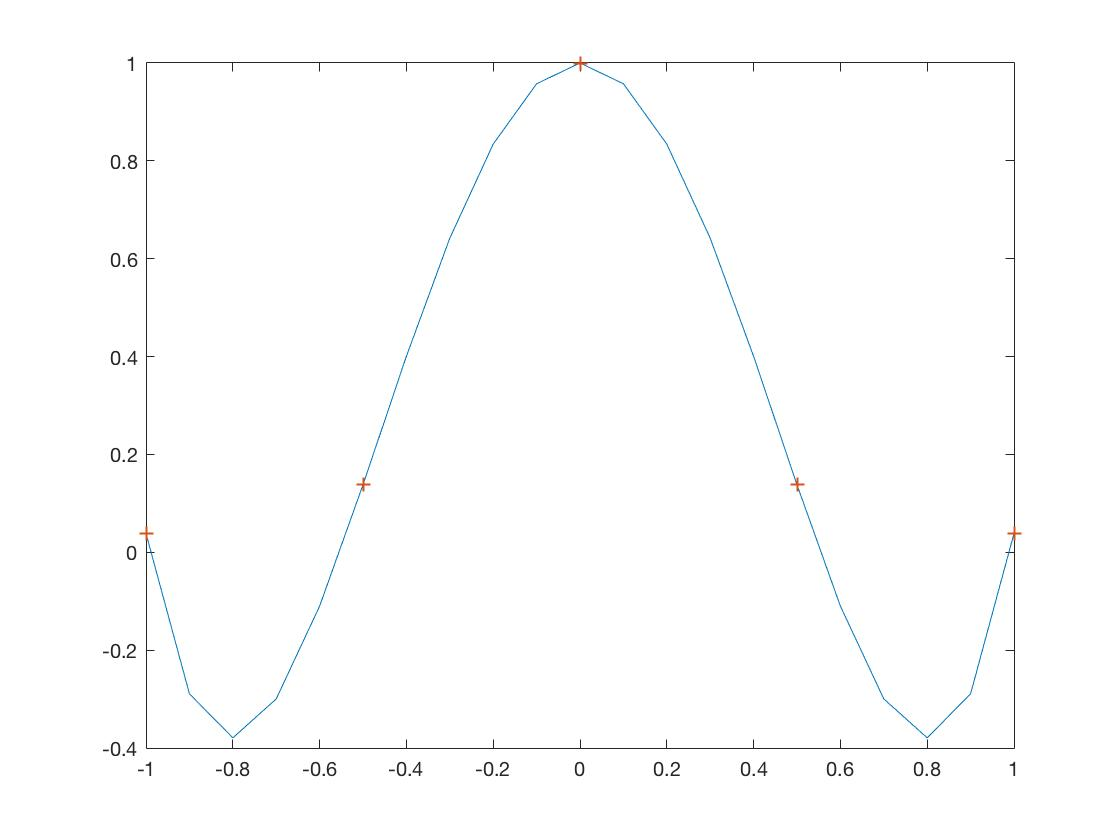
\includegraphics[scale=0.4]{Problem_3_n=5}
\end{figure}

\begin{figure}[H]
\centering
\caption{Polynomial interpolation when n = 10}
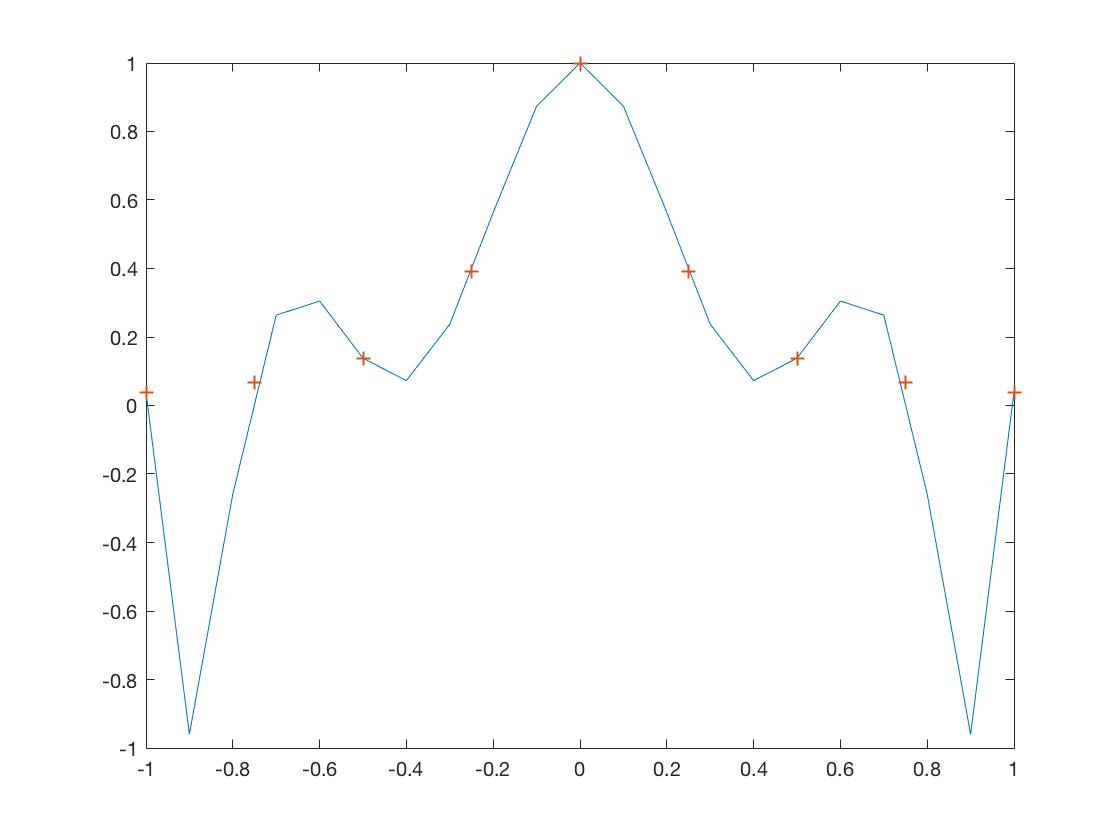
\includegraphics[scale=0.4]{Problem_3_n=10}
\end{figure}

\begin{figure}[H]
\centering
\caption{Polynomial interpolation when n = 15}
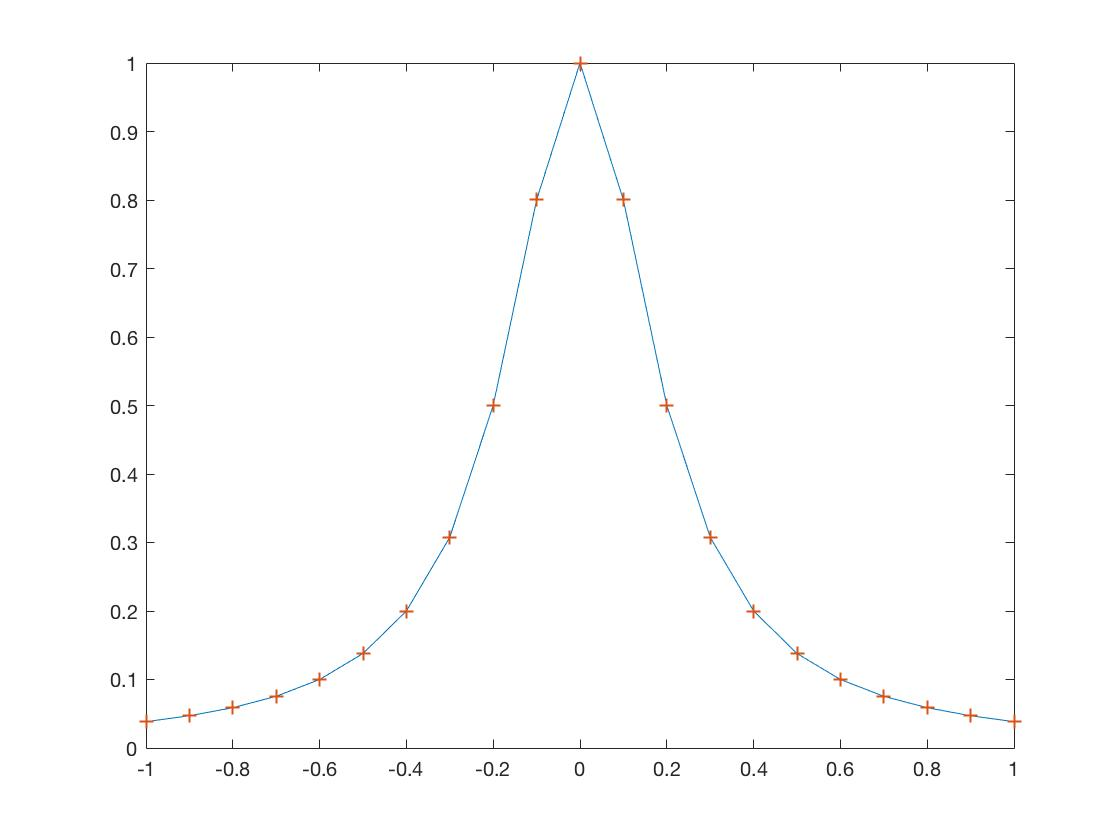
\includegraphics[scale=0.4]{Problem_3_n=15}
\end{figure}

\begin{figure}[H]
\centering
\caption{The graph of f(x)}
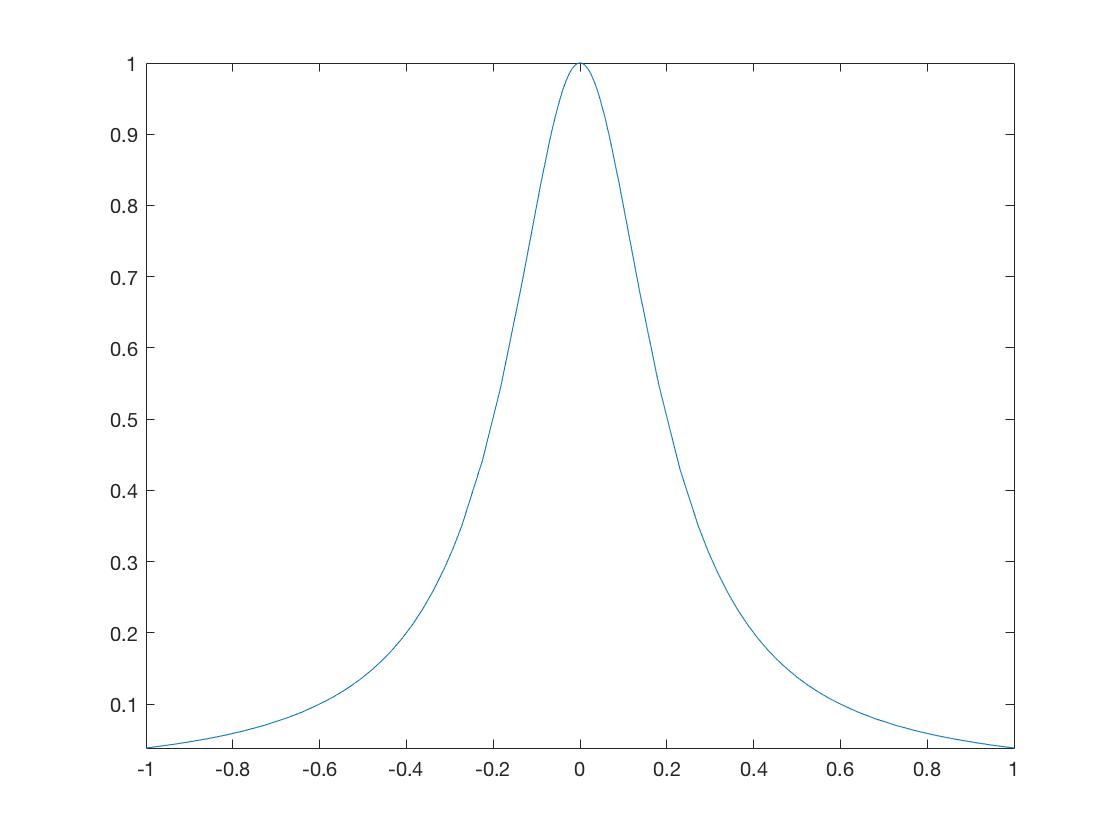
\includegraphics[scale=0.4]{Problem_3_actual}
\end{figure}



\end{document}
